\documentclass[aspectratio=169]{beamer}

\usepackage{cancel}
\usepackage{systeme}

\title[Atmospheric Effects]{Atmospheric effects for gorund-based CMB observations}
\author[Mandelli S.]{Stefano Mandelli \\ \texttt{stefano.mandelli@unimi.it}}

\date[STRIPConf]{24 - June - 2020}
\institute[UNIMI - INFN]{Universit\`a degli Studi di Milano - Istituto Nazionale di Fisica Nucleare}

\titlegraphic{
\includegraphics[scale=0.03]{ASI.png}
\includegraphics[scale=0.03]{INFN.png}\,\,\,\,\,
\includegraphics[scale=0.025]{UNIMI.png}}

%\usetheme{AnnArbor}
\usetheme{Madrid}
%\usetheme{Warsaw}
%\usetheme{Copenhagen}
\useoutertheme[top]{sidebar}
\setbeamercovered{dynamic}
%\usecolortheme{albatross}
\usecolortheme{beetle}
%\usecolortheme{crane}
%\usecolortheme{dove}


\definecolor{airforceblue}{rgb}{0.36, 0.54, 0.66}
\definecolor{asparagus}{rgb}{0.53, 0.6, 0.42}
\definecolor{carmine}{rgb}{0.8, 0.0, 0.22}

%\setbeamertemplate{blocks}[rounded][shadow=false]
%\addtobeamertemplate{block begin}{\pgfsetfillopacity{0.8}}{\pgfsetfillopacity{1}}

\setbeamercolor*{block title}{fg=white, bg=airforceblue}
\setbeamercolor*{block body}{bg=lightgray, fg=black}

\setbeamercolor*{block title example}{fg=white, bg=asparagus}
\setbeamercolor*{block body example}{bg=lightgray, fg=black}

\setbeamercolor*{block title alerted}{fg=white, bg=carmine}
\setbeamercolor*{block body alerted}{bg=lightgray, fg=black}

\begin{document}

\begin{frame}
	\maketitle
\end{frame}

\begin{frame}
    \frametitle{Index}
    \centering
    \tableofcontents
\end{frame}

\section{Introduction}
\begin{frame}
    \frametitle{The atmosphere's role in the CMB observation}
    \onslide<1->\begin{block}{Atmospheric load in the microwave band}
        \begin{itemize}[<+->]
            \item Due to absorption / emission processes
            \begin{itemize}
                \item Water vapor
                \item Oxygen molecules
            \end{itemize}
            \item The oxygen is well mixed in the atmosphere
            \begin{itemize}
                \item The increase of the optical load led to an increasing in the white noise level
            \end{itemize}
            \item The water vapor presents highly variable concentrations
            \begin{itemize}
                \item spurious $1/f$-like noise in the time-streams
            \end{itemize}
        \end{itemize}
    \end{block}

    \onslide<8->\begin{alertblock}{Assessment of the scientific impact}
        We have to create a model of the atmosphere and simulate its observation. We can start from the atmospheric dispersive proprieties
    \end{alertblock}


\end{frame}

\section{The Model}
\begin{frame}
    \frametitle{The atmosphere as a dispersive medium}
    \begin{columns}
        \onslide<1->\begin{column}{0.6\textwidth}
            \begin{itemize}[<+->]
                \item Dispersive medium: $\varepsilon(\omega) = \varepsilon(\omega)_R + i \,\varepsilon(\omega)_I$

                \item The contribute to complex permittivity are due mostly to the water vapor and the oxygen molecules that are dissolved in the atmosphere

                \item $\varepsilon(\omega)_R = \sqrt{n}$, and $\varepsilon(\omega)_I = \lambda \alpha /  4 \pi$
                \item The real and complex parts of $\varepsilon(\omega)$ are linked by the Kramers-Kr\"onig relations.
                \item There is a relation also between the refractive index $n$ and the apsorption coefficient $\alpha$
            \end{itemize}
        \end{column}
        \onslide<1->\begin{column}{0.4\textwidth}
            \onslide<5->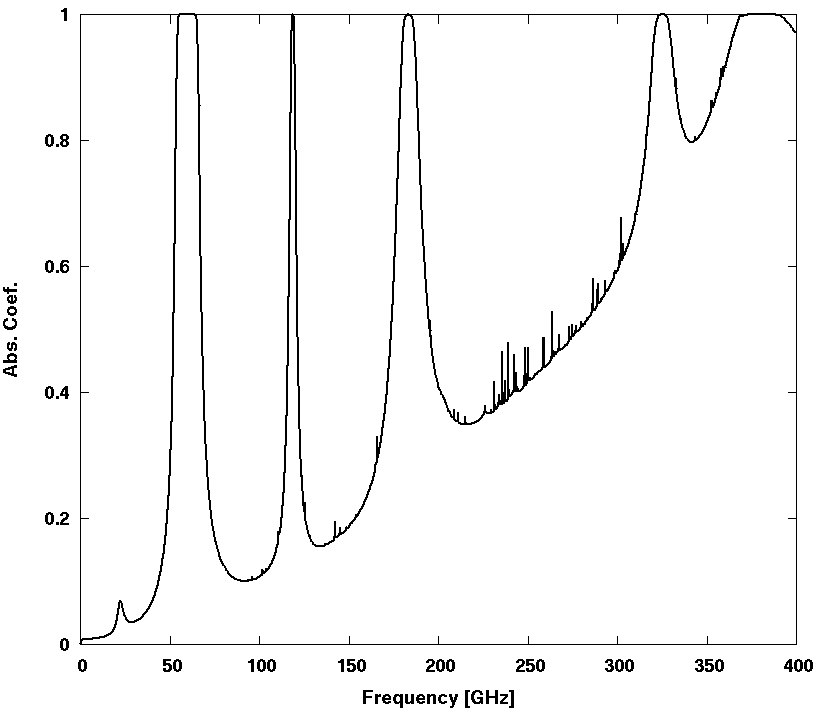
\includegraphics[scale=0.18]{Abs_Coef.jpg}
        \end{column}
    \end{columns}
\end{frame}


\begin{frame}
    \frametitle{Fluctuations in the refractive index}
    \onslide<1->Refractive index fluctuations induce a change in the optical path length, and leds a two different systematic effects for interferometry or single dish, relatively
    \begin{columns}
        \begin{column}{0.55\textwidth}
            \centering
            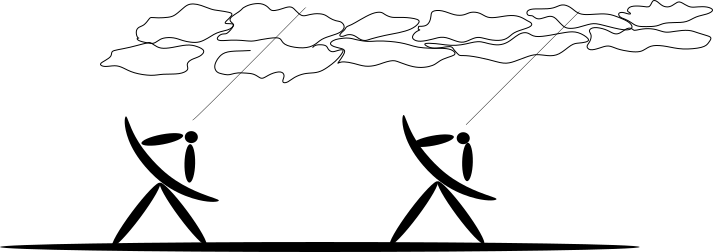
\includegraphics[scale=0.4]{path32.png}
            \textbf{Interferometer:} Phase fluctuations, degrade the interference pattern.
        \end{column}
        \begin{column}{0.45\textwidth}
            \centering
            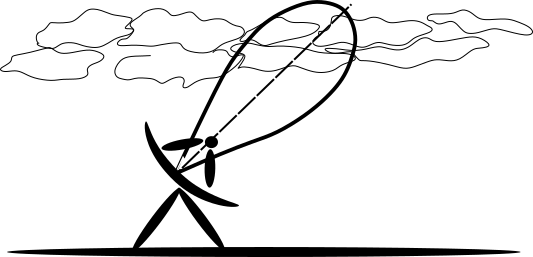
\includegraphics[scale=0.4]{path33.png}
            \textbf{Single-dish:} can cause fluctuations in the apparent pointing
        \end{column}

    \end{columns}
    \onslide<2->\begin{alertblock}{An interesting power-low relation}
        There is a relations between the RMS phase fluctuations and the interference baseline $\langle\phi^2\rangle \sim D ^{5/3}$ [see S.E. Church paper]
    \end{alertblock}
\end{frame}

\begin{frame}
    \frametitle{Fluctuations in the absorption coefficient}
    \begin{columns}
        \begin{column}{0.65\textwidth}
            \begin{itemize}[<+->]
                \item Atmospheric brightness temperature is related to $\alpha$: \only<1>{$T_B=\int_0^R\alpha(r)T_p(r)e^{-\tau'}\,dr$}\only<2-> {$T_B=\int_0^R\alpha(r)T_p(r)\cancel{e^{-\tau'}}\,dr$}
                \item $e^{-\tau} \sim 1$, $\tau$ fluctuations are small compared to $\alpha$
                \item Antenna temperature: $T_A = \frac{1}{\lambda^2}\int_V A(\hat{r}_s, \vec{r})T_p(\vec{r})\frac{dV}{r^2}$
            \end{itemize}
        \end{column}
        \begin{column}{0.35\textwidth}
            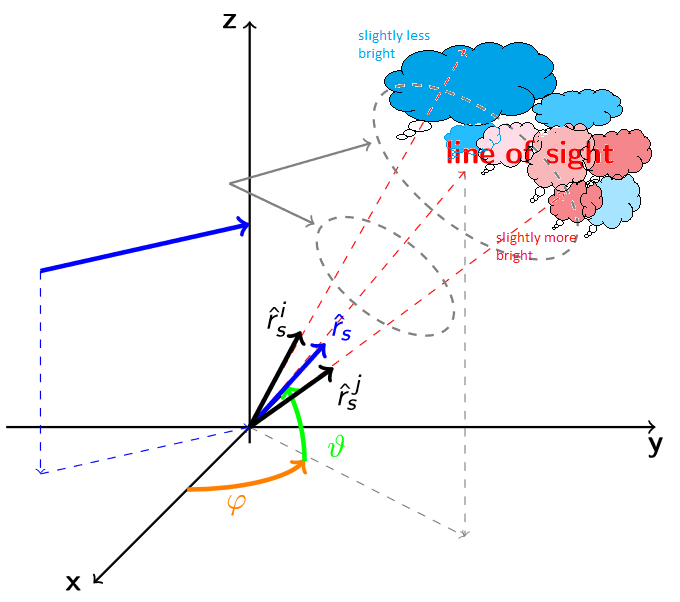
\includegraphics[scale=0.2]{Atmosphere.png}
        \end{column}
    \end{columns}

    \onslide<4->\begin{equation}
        \langle T_A^2 \rangle = \frac{1}{\lambda^4}\int_V \frac{dV}{r^2}\int_{V'}\frac{dV'}{r'^2} A(\hat{r}_s, \vec{r})A(\hat{r'}_s, \vec{r'})T_p(\vec{r})T_p(\vec{r'})\langle\alpha(\vec{r}), \alpha(\vec{r'})\rangle\nonumber
    \end{equation}

    \begin{alertblock}{Atmosphere structures}
        \centering
        The correlation term $\langle\alpha(r), \alpha(r')\rangle$ is unknown.
    \end{alertblock}

\end{frame}

\begin{frame}
    \frametitle{Characterizing the turbulent structure of the atmosphere}
    \framesubtitle{\textcolor{gray}{Interferometric observation of the atmospheric structures}}
    \begin{columns}
        \begin{column}{0.75\textwidth}
            \begin{itemize}[<+->]
                \item Structural spatial function $D_n(r_1, r_2)=\langle[n(r_1)-n(r_2)]^2\rangle$
                \item Inner and outer correlation lengths $l_0$ and $L_0$
                \item Specific humidity $q$
                    \begin{itemize}
                        \item Liquid (TQL)
                        \item Ice cristals (TQI)
                        \item Precipitable water vapor (TQV)
                    \end{itemize}
                \item Ground temperature $T_0$
                \item Solar irradiation
                \item Wind speed and direction
            \end{itemize}
        \end{column}
        \begin{column}{0.25\textwidth}
            \centering
            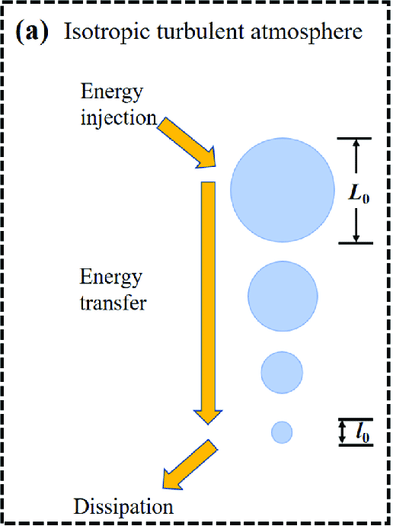
\includegraphics[scale=0.4]{Energy.png}
        \end{column}
    \end{columns}
    \onslide<10->\begin{exampleblock}{Structural spatial function for $n$}
        \begin{equation}
            \onslide<10->D(r_1, r_2) \propto L_0^{4/3} \left(\frac{dn}{dq}\frac{dq}{dz}\right)\lvert r_1 - r_2\rvert^{2/3} \propto C_0^2 \exp\left(-\frac{z}{z_0}\right)\nonumber
        \end{equation}
    \end{exampleblock}
\end{frame}

\begin{frame}
    \frametitle{Characterizing the turbulent structure of the atmosphere}
    \framesubtitle{\textcolor{gray}{The structural spatial function for the atmospheric absorption coefficient}}
    \begin{itemize}[<+->]
        \item The refractive index and the absorption coefficient are linked by the KK relations
        \item Same dependency from the atmospheric humidity $q$
        \item We can neglect second order term and consider $D_n = D_\alpha$
    \end{itemize}
    \onslide<4->$D_\alpha(r_1,r_2) = \langle[\alpha(r_1)-\alpha(r_2)]^2\rangle$, using the correlation $B_\alpha(r_1, r_2) = \langle\alpha(r_1), \alpha(r_2)\rangle$
    \onslide<5->\begin{equation}
        \begin{split}
            D_\alpha(r_1, r_2)&=\langle[\alpha(r_1) -\alpha(r_2)]^2\rangle = B_\alpha(r_1, r_1) + B_\alpha(r_2, r_2) - 2\,B_\alpha(r_1, r_2)  = \\
            &=C_\alpha^2\left(\frac{r_1+r_2}{2}\right)\lvert r_1 - r_2\rvert^{2/3}
        \end{split}\nonumber
    \end{equation}

    \onslide<6->\begin{equation}
        B_\alpha(r_1, r_2) = \frac{1}{2} C_\alpha^2 \left(\frac{r_1+r_2}{2}\right) L_0^{2/3}\left(1-\frac{\lvert r_1 - r_2 \rvert^{2/3}}{L_0^{2/3}}\right)\nonumber
    \end{equation}
\end{frame}

\begin{frame}
    \frametitle{Characterizing the turbulent structure of the atmosphere}
    \framesubtitle{\textcolor{gray}{The structural spatial function for the atmospheric absorption coefficient}}
    The $\langle\alpha(r_1),\alpha(r_2)\rangle$ expression
    \begin{equation}
        B_\alpha(r_1, r_2) = \frac{1}{2} C_\alpha^2 \left(\frac{r_1+r_2}{2}\right) L_0^{2/3}\left(1-\frac{\lvert r_1 - r_2 \rvert^{2/3}}{L_0^{2/3}}\right)\nonumber
    \end{equation}

    can be written more general

    \begin{equation}
        B_\alpha(r_1, r_2) = \frac{1}{2} C_\alpha^2\left(\frac{r_1+r_2}{2}\right)L_0^{2/3} b_\alpha(\lvert r_1 - r_2 \rvert)
    \end{equation}

    \onslide<2->\begin{block}{Kolmogorov-Modified power spectrum}
        \begin{equation}
            b_\alpha(r) \propto \frac{1}{r}\int_{k_0}^{k_M} k \Phi(k) \sin(k\cdot r)\,dk
        \end{equation}
    \end{block}
\end{frame}

\begin{frame}
    \frametitle{Characterizing the turbulent structure of the atmosphere}
    \framesubtitle{\textcolor{gray}{Different kind of $b_\alpha$ spectrum}}
    \onslide<1->\begin{block}{Kolmogorov-Modified power spectrum}
        \begin{equation}
            b_\alpha(r) \propto \frac{1}{r}\int_{k_0}^{k_M} k \Phi(k) \sin(k\cdot r)\,dk
        \end{equation}
    \end{block}

    \begin{columns}
        \begin{column}{0.5\textwidth}
            \begin{itemize}[<+->]
                \item Kolmogorov-Taylor model
                \begin{itemize}
                    \item $\Phi(k) \propto k^{-11/3}$
                    \item $k_0 = 1/L_0$
                    \item $k_M=1/l_0$
                \end{itemize}
                \item Gaussian-Like correlation
                \begin{itemize}
                    \item $b_\alpha(\lvert r_1 - r_2\rvert) = \exp\left[-\frac{\lvert r_1 - r_2\rvert^2}{2(L_0/3)^2}\right]$
                \end{itemize}
            \end{itemize}
        \end{column}
        \begin{column}{0.5\textwidth}
            \centering
            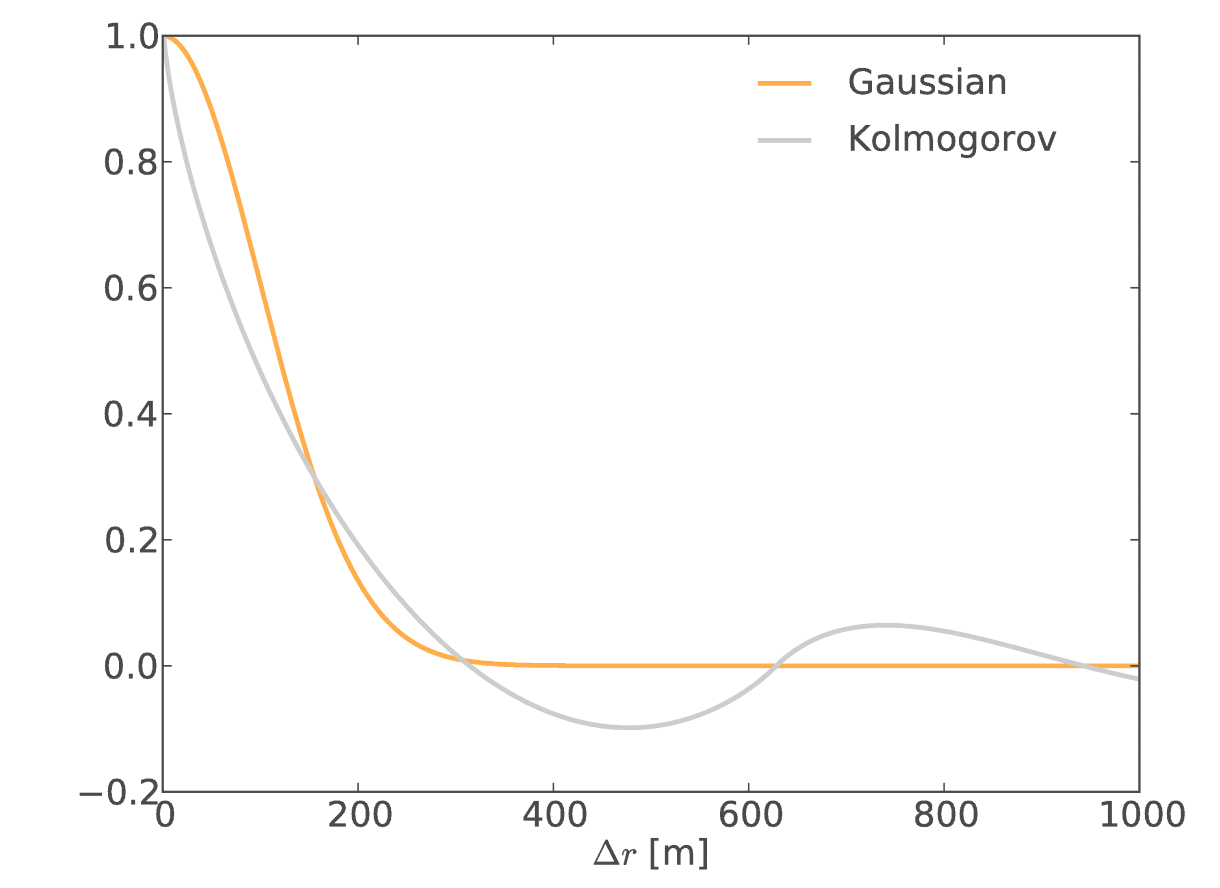
\includegraphics[scale=0.20]{Kol_Gauss.png}\\
            $L_0 = 100m$
        \end{column}

    \end{columns}
\end{frame}

\begin{frame}
    \frametitle{Temporal fluctuations in antenna temperature}
    \framesubtitle{The rigid translation of the atmospheric structures by the wind}
    \begin{equation}
        T_A(t) = \frac{1}{\lambda^2}\int_{z_1}^{z_u}\iint_{-\infty}^{+\infty}\alpha(x,y,z)T_p(z)A(x-vt,y,z)\,\frac{dx\,dy\,dz}{z^2}
    \end{equation}

    \begin{equation}
        \begin{split}
            \langle T_A(t), T_A(t+\tau) \rangle = &\frac{L_0^{2/3}}{2\pi}\int_{z_1}^{z_u}\frac{dZ}{w^2(Z)} C_\alpha^2(Z) T_p^2(Z) \iiint_{-\infty}^{+\infty}b_\alpha(\xi_x, \xi_y, \xi_z) \cdot \\
            &\cdot \exp\left[-\frac{(\xi_x+vt)^2+\xi_y^2}{w^2(Z)}\right] d\xi_x\,d\xi_y\,d\xi_z
        \end{split}
    \end{equation}

    \begin{equation}
        S(\omega) = \frac{1}{\sqrt{2\pi}} \int_{-\infty}^{+\infty} \langle T_A(t), T_A(t+\tau) \rangle \exp(-i\omega\tau)\,d\tau
    \end{equation}
\end{frame}

\begin{frame}
    \frametitle{Temporal fluctuations in antenna temperature}
    \framesubtitle{The two-slope model}
    \begin{equation}
        \begin{split}
            S(\omega) = &\frac{1}{2\sqrt{2\pi}}\frac{L^{2/3}_0}{v}\int_{z_1}^{z_u}\frac{dZ}{w(Z)}C_\alpha^2(Z)T^2_p(Z)\exp\left[-\frac{w^2(Z)\omega^2}{4v^2}\right]\cdot \\
            &\iiint_{-\infty}^{+\infty} \exp\left[\frac{i \xi_x \omega}{v}\right]\exp\left[-\frac{\xi_y^2}{w^2(Z)}\right]b_\alpha(\xi_x, \xi_y, \xi_z)\,d\xi_xd\xi_yd\xi_z
        \end{split}
    \end{equation}

    \begin{equation}
        S(\omega) = \Phi(\omega/v) \cdot I(\omega/v)
    \end{equation}

    \begin{columns}
        \begin{column}{0.5\textwidth}
            \begin{itemize}
                \item If $W(Z) \gg L_0$
                \begin{itemize}
                    \item The exponential in $\xi_y$ vary slowly compared to $b_\alpha$
                    \item Describe high altitude emission
                \end{itemize}
            \end{itemize}
        \end{column}
        \begin{column}{0.5\textwidth}
            \begin{itemize}
                \item If $W(Z) \ll L_0$
                \begin{itemize}
                    \item $b_\alpha$ vary slowly compared the exponential in $\xi_y$
                    \item Describe low altitude emission
                \end{itemize}

            \end{itemize}
        \end{column}

    \end{columns}

\end{frame}


\begin{frame}
    \frametitle{Temporal fluctuations in antenna temperature}
    \framesubtitle{The two-slope model}
    \begin{columns}
        \begin{column}{0.5\textwidth}
            \begin{itemize}
                \item If $W(Z) \gg L_0$
            \end{itemize}
            \begin{center}
                $\Phi\left(\frac{\omega}{v}\right)$ = $\left\lbrace \begin{array}{c c} \left(\frac{\omega}{v}\right)^{-11/3} & \frac{1}{L_0}\ll\left(\frac{\omega}{v}\right)\ll \frac{1}{l_0} \\ const. & \frac{\omega}{v}\ll \frac{1}{L_0} \end{array} \right.$
            \end{center}
            \begin{itemize}
                \item If $W(Z) \ll L_0$
            \end{itemize}
            \begin{center}
                $\Phi\left(\frac{\omega}{v}\right)$ = $\left\lbrace \begin{array}{c c} \left(\frac{\omega}{v}\right)^{-8/3} & \frac{1}{L_0}\ll\left(\frac{\omega}{v}\right)\ll \frac{1}{l_0} \\ const. & \frac{\omega}{v}\ll \frac{1}{L_0} \end{array} \right.$
            \end{center}
        \end{column}
        \begin{column}{0.5\textwidth}
            \centering
            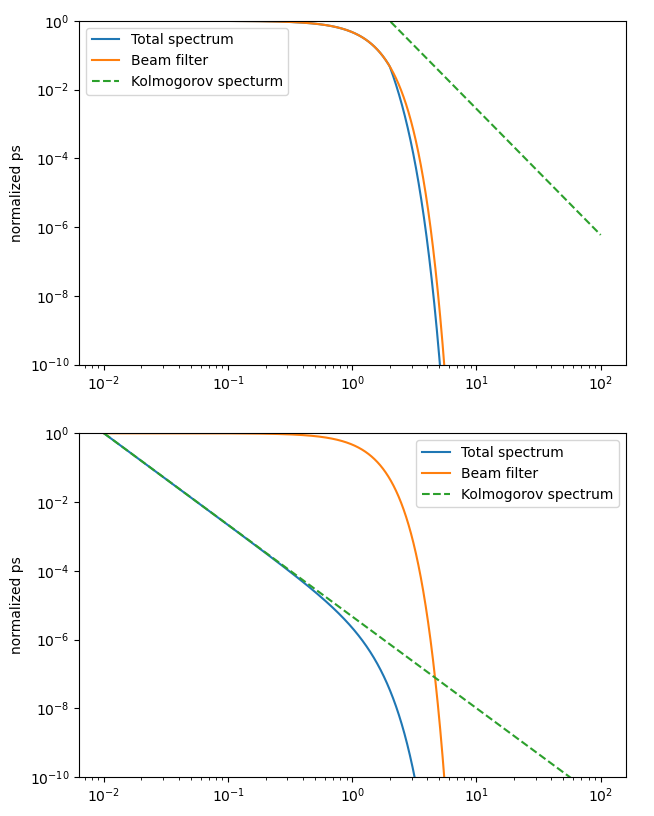
\includegraphics[scale=0.35]{Figure_1.png}
        \end{column}

    \end{columns}

\end{frame}

\section{Implementation}
\begin{frame}
    \frametitle{CAL - CMB Atmospheric Library }
\end{frame}

\section{Parameters}
\begin{frame}
    \frametitle{The statistical approach based on MERRA and ERA data}
\end{frame}




%
% \section{Un esempio}
% \begin{frame}
% 	\frametitle{Un esempio}
% 	\begin{itemize}[<+->]
% 		\item One
% 		\item Two
% 		\item Three
% 	\end{itemize}
% \end{frame}
%
% \section{Diap due}
% \begin{frame}
% 	\frametitle{Diapositiva due}
% 	\framesubtitle{Sottotitolo alla diapositiva solitamente lungo}
% \end{frame}
%
% \section{Blocchi}
% \begin{frame}
% 	\frametitle{Esempi sull'utilizzo dei Blocchi}
% 	\begin{block}{Problemi Aperti}
% 		Simulazioni...
% 	\end{block}
%
% 	\begin{exampleblock}{Esempio}
% 		Questo \`e un esempio
% 	\end{exampleblock}
%
% 	\begin{alertblock}{Errore!}
% 		Notificare errori - punti critici
% 	\end{alertblock}
%
% \end{frame}
%
% \section{Immagine}
% \begin{frame}
% 	\begin{columns}
% 		\begin{column}{0.4\textwidth}
% 			\begin{figure}
% 				\centering
% 				Immagine dell'array di Horns
% 				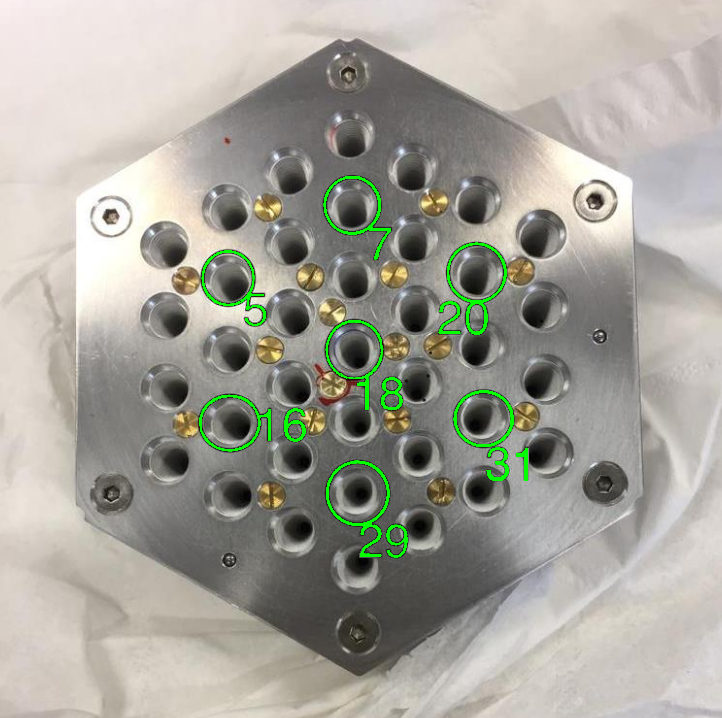
\includegraphics[scale=0.2]{Horns.png}
% 			\end{figure}
% 		\end{column}
% 		\begin{column}{0.6\textwidth}
% 			Questa \`e la descrizione all'immagine. Le didascalie alle immagini
% 			vanno sempre organizzare con colonne. Forse prima l'immagine, poi
% 			la descrizione, per una mera questione di logica.
% 		\end{column}
% 	\end{columns}
% \end{frame}





\end{document}
